% !TEX TS-program = pdflatex
% !TEX encoding = UTF-8 Unicode
\documentclass[border=0mm]{standalone}
% packages
\usepackage{tikz}
\usetikzlibrary{patterns}
\usepackage{amsmath,amssymb}
\usepackage{bm}
\usepackage{pgfplots}
\pgfplotsset{compat=1.15}
% start document
\begin{document}
% generated by ROOT (CERN)
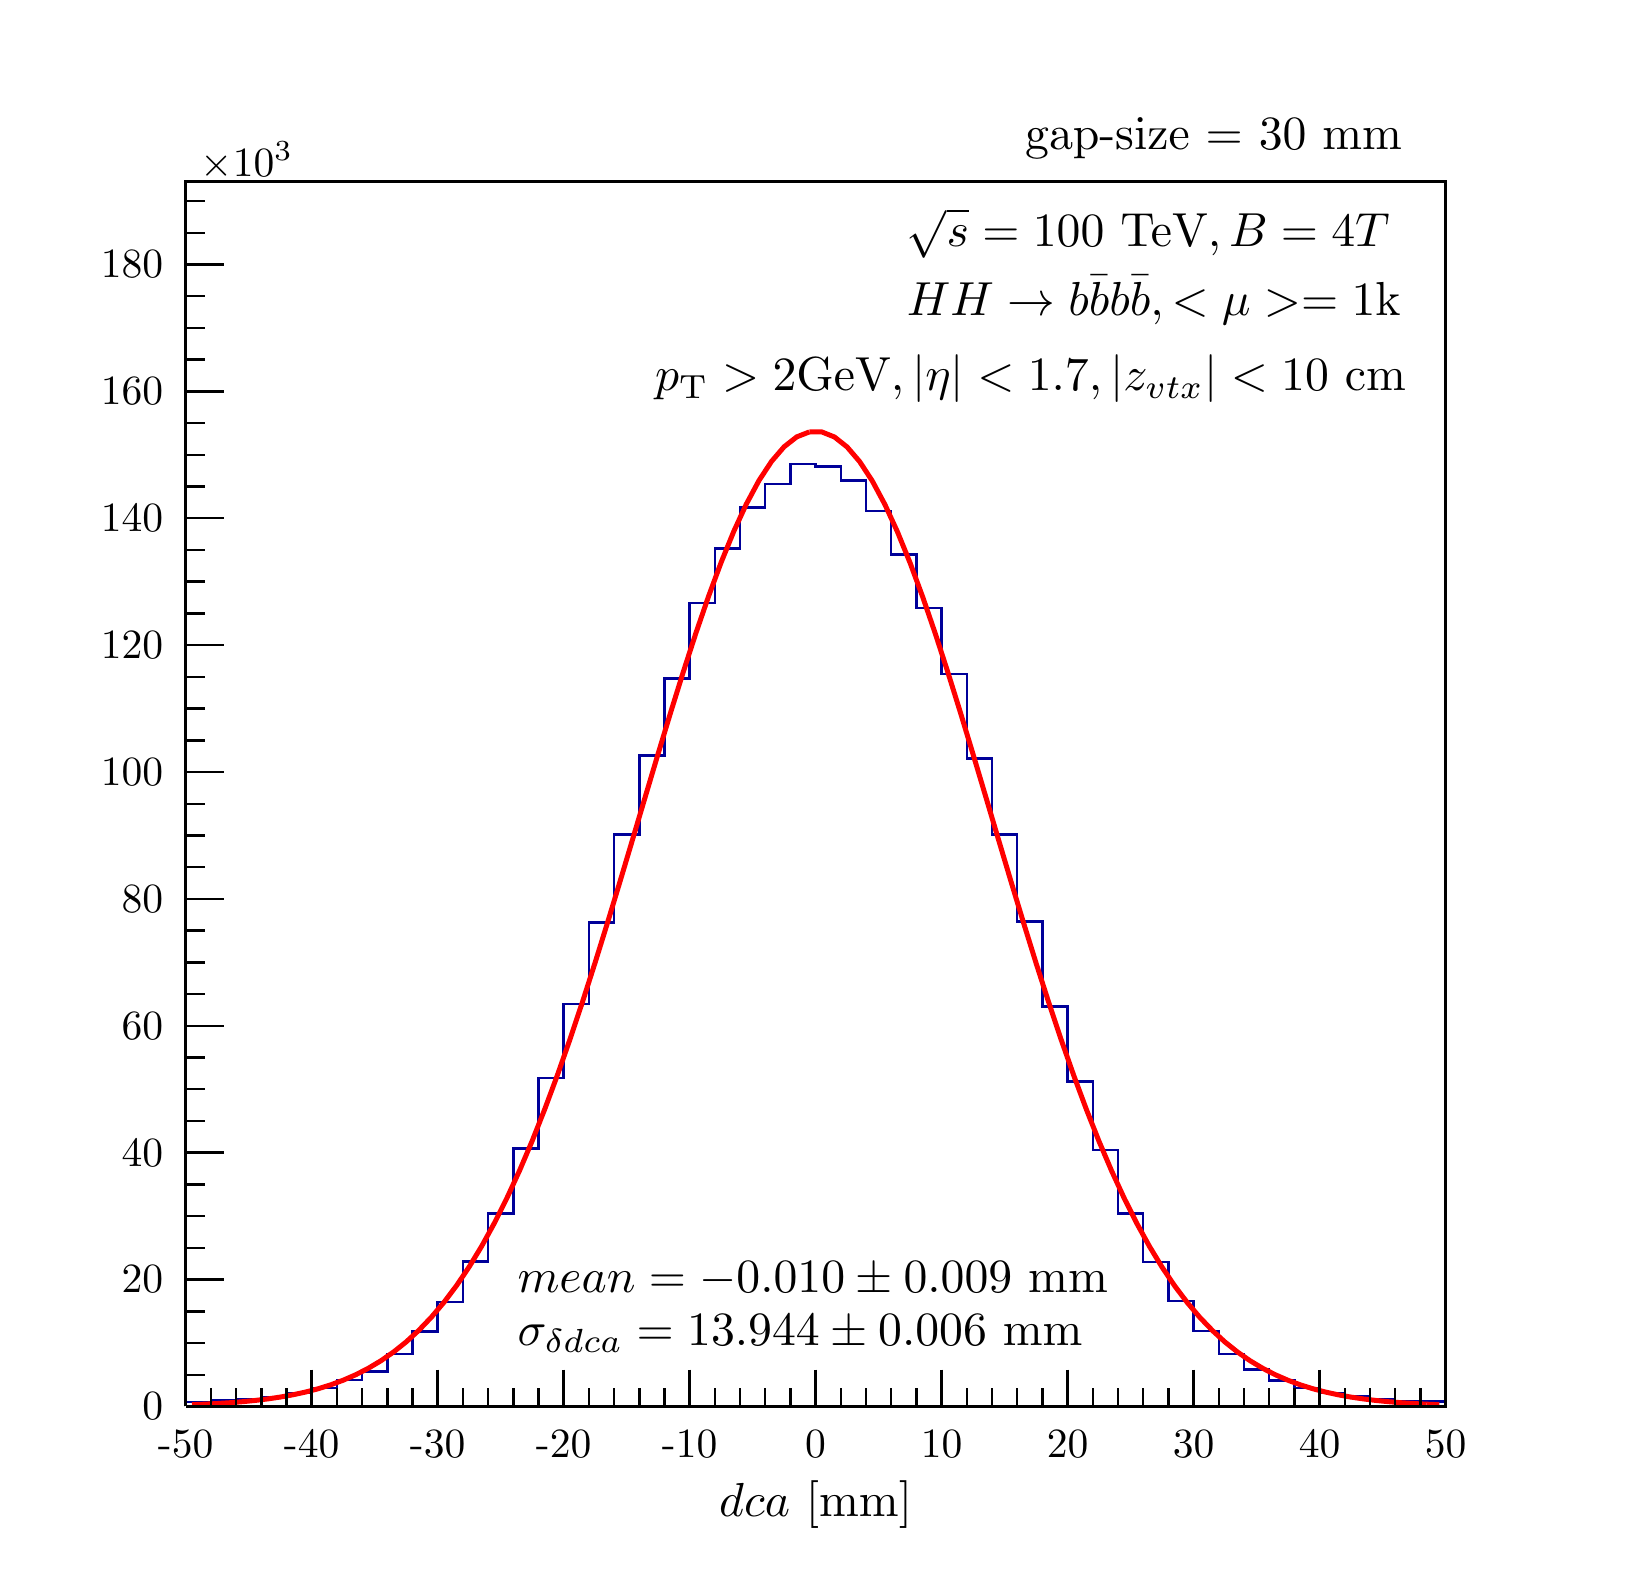
\begin{tikzpicture}
\pgfdeclareplotmark{cross} {
\pgfpathmoveto{\pgfpoint{-0.3\pgfplotmarksize}{\pgfplotmarksize}}
\pgfpathlineto{\pgfpoint{+0.3\pgfplotmarksize}{\pgfplotmarksize}}
\pgfpathlineto{\pgfpoint{+0.3\pgfplotmarksize}{0.3\pgfplotmarksize}}
\pgfpathlineto{\pgfpoint{+1\pgfplotmarksize}{0.3\pgfplotmarksize}}
\pgfpathlineto{\pgfpoint{+1\pgfplotmarksize}{-0.3\pgfplotmarksize}}
\pgfpathlineto{\pgfpoint{+0.3\pgfplotmarksize}{-0.3\pgfplotmarksize}}
\pgfpathlineto{\pgfpoint{+0.3\pgfplotmarksize}{-1.\pgfplotmarksize}}
\pgfpathlineto{\pgfpoint{-0.3\pgfplotmarksize}{-1.\pgfplotmarksize}}
\pgfpathlineto{\pgfpoint{-0.3\pgfplotmarksize}{-0.3\pgfplotmarksize}}
\pgfpathlineto{\pgfpoint{-1.\pgfplotmarksize}{-0.3\pgfplotmarksize}}
\pgfpathlineto{\pgfpoint{-1.\pgfplotmarksize}{0.3\pgfplotmarksize}}
\pgfpathlineto{\pgfpoint{-0.3\pgfplotmarksize}{0.3\pgfplotmarksize}}
\pgfpathclose
\pgfusepathqstroke
}
\pgfdeclareplotmark{cross*} {
\pgfpathmoveto{\pgfpoint{-0.3\pgfplotmarksize}{\pgfplotmarksize}}
\pgfpathlineto{\pgfpoint{+0.3\pgfplotmarksize}{\pgfplotmarksize}}
\pgfpathlineto{\pgfpoint{+0.3\pgfplotmarksize}{0.3\pgfplotmarksize}}
\pgfpathlineto{\pgfpoint{+1\pgfplotmarksize}{0.3\pgfplotmarksize}}
\pgfpathlineto{\pgfpoint{+1\pgfplotmarksize}{-0.3\pgfplotmarksize}}
\pgfpathlineto{\pgfpoint{+0.3\pgfplotmarksize}{-0.3\pgfplotmarksize}}
\pgfpathlineto{\pgfpoint{+0.3\pgfplotmarksize}{-1.\pgfplotmarksize}}
\pgfpathlineto{\pgfpoint{-0.3\pgfplotmarksize}{-1.\pgfplotmarksize}}
\pgfpathlineto{\pgfpoint{-0.3\pgfplotmarksize}{-0.3\pgfplotmarksize}}
\pgfpathlineto{\pgfpoint{-1.\pgfplotmarksize}{-0.3\pgfplotmarksize}}
\pgfpathlineto{\pgfpoint{-1.\pgfplotmarksize}{0.3\pgfplotmarksize}}
\pgfpathlineto{\pgfpoint{-0.3\pgfplotmarksize}{0.3\pgfplotmarksize}}
\pgfpathclose
\pgfusepathqfillstroke
}
\pgfdeclareplotmark{newstar} {
\pgfpathmoveto{\pgfqpoint{0pt}{\pgfplotmarksize}}
\pgfpathlineto{\pgfqpointpolar{44}{0.5\pgfplotmarksize}}
\pgfpathlineto{\pgfqpointpolar{18}{\pgfplotmarksize}}
\pgfpathlineto{\pgfqpointpolar{-20}{0.5\pgfplotmarksize}}
\pgfpathlineto{\pgfqpointpolar{-54}{\pgfplotmarksize}}
\pgfpathlineto{\pgfqpointpolar{-90}{0.5\pgfplotmarksize}}
\pgfpathlineto{\pgfqpointpolar{234}{\pgfplotmarksize}}
\pgfpathlineto{\pgfqpointpolar{198}{0.5\pgfplotmarksize}}
\pgfpathlineto{\pgfqpointpolar{162}{\pgfplotmarksize}}
\pgfpathlineto{\pgfqpointpolar{134}{0.5\pgfplotmarksize}}
\pgfpathclose
\pgfusepathqstroke
}
\pgfdeclareplotmark{newstar*} {
\pgfpathmoveto{\pgfqpoint{0pt}{\pgfplotmarksize}}
\pgfpathlineto{\pgfqpointpolar{44}{0.5\pgfplotmarksize}}
\pgfpathlineto{\pgfqpointpolar{18}{\pgfplotmarksize}}
\pgfpathlineto{\pgfqpointpolar{-20}{0.5\pgfplotmarksize}}
\pgfpathlineto{\pgfqpointpolar{-54}{\pgfplotmarksize}}
\pgfpathlineto{\pgfqpointpolar{-90}{0.5\pgfplotmarksize}}
\pgfpathlineto{\pgfqpointpolar{234}{\pgfplotmarksize}}
\pgfpathlineto{\pgfqpointpolar{198}{0.5\pgfplotmarksize}}
\pgfpathlineto{\pgfqpointpolar{162}{\pgfplotmarksize}}
\pgfpathlineto{\pgfqpointpolar{134}{0.5\pgfplotmarksize}}
\pgfpathclose
\pgfusepathqfillstroke
}
\definecolor{c}{rgb}{1,1,1};
\draw [color=c, fill=c] (0,0) rectangle (20,19.4486);
\draw [color=c, fill=c] (2,1.94486) rectangle (18,17.5038);
\definecolor{c}{rgb}{0,0,0};
\draw [c,line width=0.9] (2,1.94486) -- (2,17.5038) -- (18,17.5038) -- (18,1.94486) -- (2,1.94486);
\definecolor{c}{rgb}{1,1,1};
\draw [color=c, fill=c] (2,1.94486) rectangle (18,17.5038);
\definecolor{c}{rgb}{0,0,0};
\draw [c,line width=0.9] (2,1.94486) -- (2,17.5038) -- (18,17.5038) -- (18,1.94486) -- (2,1.94486);
\definecolor{c}{rgb}{0,0,0.6};
\draw [c,line width=0.9] (2,2.00296) -- (2.32,2.00296) -- (2.32,2.02334) -- (2.64,2.02334) -- (2.64,2.03293) -- (2.96,2.03293) -- (2.96,2.06379) -- (3.28,2.06379) -- (3.28,2.11817) -- (3.6,2.11817) -- (3.6,2.18255) -- (3.92,2.18255) -- (3.92,2.2794)
 -- (4.24,2.2794) -- (4.24,2.38745) -- (4.56,2.38745) -- (4.56,2.61442) -- (4.88,2.61442) -- (4.88,2.89756) -- (5.2,2.89756) -- (5.2,3.26908) -- (5.52,3.26908) -- (5.52,3.78797) -- (5.84,3.78797) -- (5.84,4.39823) -- (6.16,4.39823) -- (6.16,5.22362)
 -- (6.48,5.22362) -- (6.48,6.11677) -- (6.8,6.11677) -- (6.8,7.05367) -- (7.12,7.05367) -- (7.12,8.09024) -- (7.44,8.09024) -- (7.44,9.21028) -- (7.76,9.21028) -- (7.76,10.2148) -- (8.08,10.2148) -- (8.08,11.1914) -- (8.4,11.1914) -- (8.4,12.1468)
 -- (8.72,12.1468) -- (8.72,12.8435) -- (9.04,12.8435) -- (9.04,13.36) -- (9.36,13.36) -- (9.36,13.6597) -- (9.68,13.6597) -- (9.68,13.9132) -- (10,13.9132) -- (10,13.8834) -- (10.32,13.8834) -- (10.32,13.7071) -- (10.64,13.7071) -- (10.64,13.3145)
 -- (10.96,13.3145) -- (10.96,12.7636) -- (11.28,12.7636) -- (11.28,12.0842) -- (11.6,12.0842) -- (11.6,11.2494) -- (11.92,11.2494) -- (11.92,10.1743) -- (12.24,10.1743) -- (12.24,9.20763) -- (12.56,9.20763) -- (12.56,8.10087) -- (12.88,8.10087) --
 (12.88,7.02595) -- (13.2,7.02595) -- (13.2,6.06939) -- (13.52,6.06939) -- (13.52,5.19952) -- (13.84,5.19952) -- (13.84,4.39355) -- (14.16,4.39355) -- (14.16,3.77717) -- (14.48,3.77717) -- (14.48,3.28133) -- (14.8,3.28133) -- (14.8,2.90594) --
 (15.12,2.90594) -- (15.12,2.60975) -- (15.44,2.60975) -- (15.44,2.41275) -- (15.76,2.41275) -- (15.76,2.27191) -- (16.08,2.27191) -- (16.08,2.1778) -- (16.4,2.1778) -- (16.4,2.11511) -- (16.72,2.11511) -- (16.72,2.07394) -- (17.04,2.07394) --
 (17.04,2.03486) -- (17.36,2.03486) -- (17.36,2.01005) -- (17.68,2.01005) -- (17.68,2.01045) -- (18,2.01045);
\definecolor{c}{rgb}{1,0,0};
\draw [c,line width=1.8] (2.08,1.96763) -- (2.24,1.97415) -- (2.4,1.98235) -- (2.56,1.9926) -- (2.72,2.00534) -- (2.88,2.02109) -- (3.04,2.04044) -- (3.2,2.0641) -- (3.36,2.09284) -- (3.52,2.12757) -- (3.68,2.1693) -- (3.84,2.21914) -- (4,2.27833) --
 (4.16,2.34821) -- (4.32,2.43024) -- (4.48,2.52594) -- (4.64,2.63695) -- (4.8,2.76494) -- (4.96,2.91161) -- (5.12,3.07867) -- (5.28,3.26778) -- (5.44,3.4805) -- (5.6,3.71829) -- (5.76,3.98239) -- (5.92,4.27382) -- (6.08,4.59326) -- (6.24,4.94108) --
 (6.4,5.31718) -- (6.56,5.72101) -- (6.72,6.15152) -- (6.88,6.60707) -- (7.04,7.08543) -- (7.2,7.58381) -- (7.36,8.09876) -- (7.52,8.62629) -- (7.68,9.16183) -- (7.84,9.70029) -- (8,10.2362) -- (8.16,10.7636) -- (8.32,11.2765) -- (8.48,11.7685) --
 (8.64,12.2335) -- (8.8,12.6651) -- (8.96,13.0576) -- (9.12,13.4053) -- (9.28,13.7033) -- (9.44,13.9471) -- (9.6,14.1331) -- (9.76,14.2585) -- (9.92,14.3214);
\draw [c,line width=1.8] (9.92,14.3214) -- (10.08,14.3208) -- (10.24,14.2567) -- (10.4,14.1301) -- (10.56,13.943) -- (10.72,13.698) -- (10.88,13.3991) -- (11.04,13.0504) -- (11.2,12.6572) -- (11.36,12.2248) -- (11.52,11.7593) -- (11.68,11.2668) --
 (11.84,10.7536) -- (12,10.226) -- (12.16,9.68997) -- (12.32,9.15151) -- (12.48,8.61608) -- (12.64,8.08875) -- (12.8,7.57408) -- (12.96,7.07606) -- (13.12,6.59811) -- (13.28,6.14302) -- (13.44,5.71301) -- (13.6,5.3097) -- (13.76,4.93414) --
 (13.92,4.58687) -- (14.08,4.26797) -- (14.24,3.97707) -- (14.4,3.71349) -- (14.56,3.47619) -- (14.72,3.26393) -- (14.88,3.07527) -- (15.04,2.90861) -- (15.2,2.76232) -- (15.36,2.63467) -- (15.52,2.52397) -- (15.68,2.42854) -- (15.84,2.34676) --
 (16,2.2771) -- (16.16,2.2181) -- (16.32,2.16843) -- (16.48,2.12685) -- (16.64,2.09224) -- (16.8,2.0636) -- (16.96,2.04004) -- (17.12,2.02076) -- (17.28,2.00507) -- (17.44,1.99238) -- (17.6,1.98218) -- (17.76,1.97401);
\draw [c,line width=1.8] (17.76,1.97401) -- (17.92,1.96752);
\definecolor{c}{rgb}{0,0,0};
\draw [c,line width=0.9] (2,1.94486) -- (18,1.94486);
\draw [c,line width=0.9] (2,2.41163) -- (2,1.94486);
\draw [c,line width=0.9] (2.32,2.17825) -- (2.32,1.94486);
\draw [c,line width=0.9] (2.64,2.17825) -- (2.64,1.94486);
\draw [c,line width=0.9] (2.96,2.17825) -- (2.96,1.94486);
\draw [c,line width=0.9] (3.28,2.17825) -- (3.28,1.94486);
\draw [c,line width=0.9] (3.6,2.41163) -- (3.6,1.94486);
\draw [c,line width=0.9] (3.92,2.17825) -- (3.92,1.94486);
\draw [c,line width=0.9] (4.24,2.17825) -- (4.24,1.94486);
\draw [c,line width=0.9] (4.56,2.17825) -- (4.56,1.94486);
\draw [c,line width=0.9] (4.88,2.17825) -- (4.88,1.94486);
\draw [c,line width=0.9] (5.2,2.41163) -- (5.2,1.94486);
\draw [c,line width=0.9] (5.52,2.17825) -- (5.52,1.94486);
\draw [c,line width=0.9] (5.84,2.17825) -- (5.84,1.94486);
\draw [c,line width=0.9] (6.16,2.17825) -- (6.16,1.94486);
\draw [c,line width=0.9] (6.48,2.17825) -- (6.48,1.94486);
\draw [c,line width=0.9] (6.8,2.41163) -- (6.8,1.94486);
\draw [c,line width=0.9] (7.12,2.17825) -- (7.12,1.94486);
\draw [c,line width=0.9] (7.44,2.17825) -- (7.44,1.94486);
\draw [c,line width=0.9] (7.76,2.17825) -- (7.76,1.94486);
\draw [c,line width=0.9] (8.08,2.17825) -- (8.08,1.94486);
\draw [c,line width=0.9] (8.4,2.41163) -- (8.4,1.94486);
\draw [c,line width=0.9] (8.72,2.17825) -- (8.72,1.94486);
\draw [c,line width=0.9] (9.04,2.17825) -- (9.04,1.94486);
\draw [c,line width=0.9] (9.36,2.17825) -- (9.36,1.94486);
\draw [c,line width=0.9] (9.68,2.17825) -- (9.68,1.94486);
\draw [c,line width=0.9] (10,2.41163) -- (10,1.94486);
\draw [c,line width=0.9] (10.32,2.17825) -- (10.32,1.94486);
\draw [c,line width=0.9] (10.64,2.17825) -- (10.64,1.94486);
\draw [c,line width=0.9] (10.96,2.17825) -- (10.96,1.94486);
\draw [c,line width=0.9] (11.28,2.17825) -- (11.28,1.94486);
\draw [c,line width=0.9] (11.6,2.41163) -- (11.6,1.94486);
\draw [c,line width=0.9] (11.92,2.17825) -- (11.92,1.94486);
\draw [c,line width=0.9] (12.24,2.17825) -- (12.24,1.94486);
\draw [c,line width=0.9] (12.56,2.17825) -- (12.56,1.94486);
\draw [c,line width=0.9] (12.88,2.17825) -- (12.88,1.94486);
\draw [c,line width=0.9] (13.2,2.41163) -- (13.2,1.94486);
\draw [c,line width=0.9] (13.52,2.17825) -- (13.52,1.94486);
\draw [c,line width=0.9] (13.84,2.17825) -- (13.84,1.94486);
\draw [c,line width=0.9] (14.16,2.17825) -- (14.16,1.94486);
\draw [c,line width=0.9] (14.48,2.17825) -- (14.48,1.94486);
\draw [c,line width=0.9] (14.8,2.41163) -- (14.8,1.94486);
\draw [c,line width=0.9] (15.12,2.17825) -- (15.12,1.94486);
\draw [c,line width=0.9] (15.44,2.17825) -- (15.44,1.94486);
\draw [c,line width=0.9] (15.76,2.17825) -- (15.76,1.94486);
\draw [c,line width=0.9] (16.08,2.17825) -- (16.08,1.94486);
\draw [c,line width=0.9] (16.4,2.41163) -- (16.4,1.94486);
\draw [c,line width=0.9] (16.72,2.17825) -- (16.72,1.94486);
\draw [c,line width=0.9] (17.04,2.17825) -- (17.04,1.94486);
\draw [c,line width=0.9] (17.36,2.17825) -- (17.36,1.94486);
\draw [c,line width=0.9] (17.68,2.17825) -- (17.68,1.94486);
\draw [c,line width=0.9] (18,2.41163) -- (18,1.94486);
\draw [anchor=base] (2,1.30306) node[scale=1.50291, color=c, rotate=0]{-50};
\draw [anchor=base] (3.6,1.30306) node[scale=1.50291, color=c, rotate=0]{-40};
\draw [anchor=base] (5.2,1.30306) node[scale=1.50291, color=c, rotate=0]{-30};
\draw [anchor=base] (6.8,1.30306) node[scale=1.50291, color=c, rotate=0]{-20};
\draw [anchor=base] (8.4,1.30306) node[scale=1.50291, color=c, rotate=0]{-10};
\draw [anchor=base] (10,1.30306) node[scale=1.50291, color=c, rotate=0]{0};
\draw [anchor=base] (11.6,1.30306) node[scale=1.50291, color=c, rotate=0]{10};
\draw [anchor=base] (13.2,1.30306) node[scale=1.50291, color=c, rotate=0]{20};
\draw [anchor=base] (14.8,1.30306) node[scale=1.50291, color=c, rotate=0]{30};
\draw [anchor=base] (16.4,1.30306) node[scale=1.50291, color=c, rotate=0]{40};
\draw [anchor=base] (18,1.30306) node[scale=1.50291, color=c, rotate=0]{50};
\draw (10,0.700151) node[scale=1.72557, color=c, rotate=0]{$dca$~[\text{mm}]};
\draw [c,line width=0.9] (2,1.94486) -- (2,17.5038);
\draw [c,line width=0.9] (2.48,1.94486) -- (2,1.94486);
\draw [c,line width=0.9] (2.24,2.34773) -- (2,2.34773);
\draw [c,line width=0.9] (2.24,2.75059) -- (2,2.75059);
\draw [c,line width=0.9] (2.24,3.15346) -- (2,3.15346);
\draw [c,line width=0.9] (2.48,3.55632) -- (2,3.55632);
\draw [c,line width=0.9] (2.24,3.95919) -- (2,3.95919);
\draw [c,line width=0.9] (2.24,4.36205) -- (2,4.36205);
\draw [c,line width=0.9] (2.24,4.76491) -- (2,4.76491);
\draw [c,line width=0.9] (2.48,5.16778) -- (2,5.16778);
\draw [c,line width=0.9] (2.24,5.57064) -- (2,5.57064);
\draw [c,line width=0.9] (2.24,5.97351) -- (2,5.97351);
\draw [c,line width=0.9] (2.24,6.37637) -- (2,6.37637);
\draw [c,line width=0.9] (2.48,6.77924) -- (2,6.77924);
\draw [c,line width=0.9] (2.24,7.1821) -- (2,7.1821);
\draw [c,line width=0.9] (2.24,7.58497) -- (2,7.58497);
\draw [c,line width=0.9] (2.24,7.98783) -- (2,7.98783);
\draw [c,line width=0.9] (2.48,8.3907) -- (2,8.3907);
\draw [c,line width=0.9] (2.24,8.79356) -- (2,8.79356);
\draw [c,line width=0.9] (2.24,9.19643) -- (2,9.19643);
\draw [c,line width=0.9] (2.24,9.59929) -- (2,9.59929);
\draw [c,line width=0.9] (2.48,10.0022) -- (2,10.0022);
\draw [c,line width=0.9] (2.24,10.405) -- (2,10.405);
\draw [c,line width=0.9] (2.24,10.8079) -- (2,10.8079);
\draw [c,line width=0.9] (2.24,11.2107) -- (2,11.2107);
\draw [c,line width=0.9] (2.48,11.6136) -- (2,11.6136);
\draw [c,line width=0.9] (2.24,12.0165) -- (2,12.0165);
\draw [c,line width=0.9] (2.24,12.4193) -- (2,12.4193);
\draw [c,line width=0.9] (2.24,12.8222) -- (2,12.8222);
\draw [c,line width=0.9] (2.48,13.2251) -- (2,13.2251);
\draw [c,line width=0.9] (2.24,13.6279) -- (2,13.6279);
\draw [c,line width=0.9] (2.24,14.0308) -- (2,14.0308);
\draw [c,line width=0.9] (2.24,14.4337) -- (2,14.4337);
\draw [c,line width=0.9] (2.48,14.8365) -- (2,14.8365);
\draw [c,line width=0.9] (2.24,15.2394) -- (2,15.2394);
\draw [c,line width=0.9] (2.24,15.6423) -- (2,15.6423);
\draw [c,line width=0.9] (2.24,16.0451) -- (2,16.0451);
\draw [c,line width=0.9] (2.48,16.448) -- (2,16.448);
\draw [c,line width=0.9] (2.48,16.448) -- (2,16.448);
\draw [c,line width=0.9] (2.24,16.8509) -- (2,16.8509);
\draw [c,line width=0.9] (2.24,17.2537) -- (2,17.2537);
\draw [anchor= east] (1.9,1.94486) node[scale=1.50291, color=c, rotate=0]{0};
\draw [anchor= east] (1.9,3.55632) node[scale=1.50291, color=c, rotate=0]{20};
\draw [anchor= east] (1.9,5.16778) node[scale=1.50291, color=c, rotate=0]{40};
\draw [anchor= east] (1.9,6.77924) node[scale=1.50291, color=c, rotate=0]{60};
\draw [anchor= east] (1.9,8.3907) node[scale=1.50291, color=c, rotate=0]{80};
\draw [anchor= east] (1.9,10.0022) node[scale=1.50291, color=c, rotate=0]{100};
\draw [anchor= east] (1.9,11.6136) node[scale=1.50291, color=c, rotate=0]{120};
\draw [anchor= east] (1.9,13.2251) node[scale=1.50291, color=c, rotate=0]{140};
\draw [anchor= east] (1.9,14.8365) node[scale=1.50291, color=c, rotate=0]{160};
\draw [anchor= east] (1.9,16.448) node[scale=1.50291, color=c, rotate=0]{180};
\draw [anchor=base west] (2,17.5718) node[scale=1.50291, color=c, rotate=0]{$\times10^{3}$};
\draw [anchor=base west] (6,3.39622) node[scale=1.72557, color=c, rotate=0]{$mean = -0.010 \pm 0.009 \text{~mm}$};
\draw [anchor=base west] (6,2.71551) node[scale=1.72557, color=c, rotate=0]{$\sigma_{\delta dca} = 13.944 \pm 0.006 \text{~mm}$};
\draw [anchor=base west] (10.945,16.6748) node[scale=1.72557, color=c, rotate=0]{$\sqrt{s} = 100 ~\text{TeV}, B = 4T$};
\draw [anchor=base west] (10.945,15.7996) node[scale=1.72557, color=c, rotate=0]{$HH \rightarrow b\bar{b}b\bar{b}, <\mu> = \text{1k}$};
\draw [anchor=base east] (17.7105,14.8432) node[scale=1.72557, color=c, rotate=0]{$p_{\text{T}} > 2\text{GeV}, |\eta| < 1.7, |z_{vtx}| < 10\text{~cm}$};
\draw [anchor=base west] (12.445,17.9122) node[scale=1.72557, color=c, rotate=0]{gap-size = 30 mm};
\draw [anchor=base west] (12.445,17.5232) node[scale=1.72557, color=c, rotate=0]{ };
\end{tikzpicture}
% end document
\end{document}
